%% Supplementary Material (Version 4): HSM — Proofs of 4 Lemmas + 6 Theorems
%% Paper: "Multi-Scale Workload Similarity Measurement for Proactive
%%          Database Index Tuning Using Hierarchical Signal Processing"
%% Author: Arun Reungsilpkolkarn
%% Restructured to match Version 4 (6 Theorems + 4 Lemmas) of the main paper.

\documentclass[10pt,twocolumn,a4paper]{article}
\usepackage[a4paper,top=19mm,bottom=24mm,left=14.5mm,right=14.5mm,columnsep=5mm]{geometry}
\usepackage[T1]{fontenc}
\usepackage[utf8]{inputenc}
\usepackage{amsmath,amssymb,amsthm}
\usepackage{mathtools}
\usepackage{booktabs}
\usepackage{multirow}
\usepackage{graphicx}
\usepackage{times}
\usepackage{microtype}
\usepackage[hidelinks]{hyperref}
\usepackage{placeins}
\usepackage{titlesec}
\titleformat{\section}{\bfseries\normalsize}{\Roman{section}.}{0.5em}{}
\titleformat{\subsection}{\bfseries\itshape\small}{\Alph{subsection}.}{0.4em}{}
\setlength\parindent{7pt}\setlength\parskip{0pt}
\titlespacing*{\section}{0pt}{4pt}{2pt}
\titlespacing*{\subsection}{0pt}{3pt}{1pt}

%% Theorem environments
\newtheorem{theorem}{Theorem}
\newtheorem{lemma}{Lemma}
\newtheorem{corollary}{Corollary}
\newtheorem{proposition}{Proposition}
\newtheorem{definition}{Definition}
\newtheorem{remark}{Remark}

%% HSM shorthand commands (identical to main paper)
\newcommand{\SHSM}{S_{\mathrm{HSM}}}
\newcommand{\SR}{S_{R}}
\newcommand{\SV}{S_{V}}
\newcommand{\ST}{S_{T}}
\newcommand{\SA}{S_{A}}
\newcommand{\SPER}{S_{P}}
\newcommand{\Npts}{N_{\mathrm{pts}}}
\newcommand{\Nstar}{N^{*}_{\mathrm{pts}}}
\newcommand{\dHSM}{d_{\mathrm{HSM}}}
\newcommand{\thetastar}{\theta^{*}}
\newcommand{\Cdb}{C_{\mathrm{db4}}}
\newcommand{\TPR}{\mathrm{TPR}}
\newcommand{\TNR}{\mathrm{TNR}}

\begin{document}

\twocolumn[{\begin{center}
{\large\bfseries Supplementary Material (Option D)}\\[2pt]
{\normalsize\bfseries Multi-Scale Workload Similarity Measurement for
Proactive Database Index Tuning Using Hierarchical Signal Processing}\\[4pt]
{\normalsize Arun Reungsilpkolkarn}\\
{\small School of Information Technology and Innovation, Bangkok University, Thailand.
\texttt{arun.r@bu.ac.th}}\\[4pt]
\end{center}
\begin{quote}\small
This document provides complete proofs for the four supporting lemmas
(L1--L4) and the six core theorems (T1--T6) stated in Section~IV
of the main paper, followed by extended experimental details
(Section~XI) including full A1--A7 results, A-CE protocol, extended
proof sketches, remarks, and deployment guidelines. Notation follows the main paper exactly. The five HSM
dimensions are: $\SR$ (query-template rank correlation via Spearman's
$\rho_s$, mapped through $1{-}\arccos(\rho_s)/\pi$), $\SV$ (volume
ratio), $\ST$ (query-template angular distance,
$1{-}(2/\pi)\arccos(\hat{\mathbf{v}}_A\cdot\hat{\mathbf{v}}_B)$),
$\SA$ (attribute-set Jaccard), $\SPER$ (DWT-based temporal pattern).
All five similarity functions lie in $[0,1]$; the induced distances
$d_i=1-S_i$ all satisfy the triangle inequality analytically (Lemma~1,
property P4). The composite score is
$\SHSM(W_A,W_B)=\sum_i w_i S_i(W_A,W_B)$ with default weights
$w_R\!=\!0.25$, $w_V\!=\!w_T\!=\!w_A\!=\!0.20$, $w_P\!=\!0.15$.
$\dHSM=1-\SHSM$ denotes the corresponding distance.
$\Npts=|W_A|+|W_B|$ denotes the total query events across both
windows.
\end{quote}\vspace{4pt}}]

%%─────────────────────────────────────────────────────────────
\section{Proof of Lemma~1 (HSM Metric Properties)}
%%─────────────────────────────────────────────────────────────

\begin{lemma}[HSM Metric Properties]
$\forall\,W_i,W_j,W_k\in\mathcal{W}$:
\begin{align*}
&(P1)\;\SHSM(W_i,W_j)\in[0,1];\\
&(P2)\;\SHSM(W_i,W_i)=1;\\
&(P3)\;\SHSM(W_i,W_j)=\SHSM(W_j,W_i);\\
&(P4)\;1{-}\SHSM(W_i,W_k)\leq(1{-}\SHSM(W_i,W_j))\\
&\qquad\quad+(1{-}\SHSM(W_j,W_k)).
\end{align*}
\end{lemma}

\begin{proof}
We verify each property in turn.

\textbf{P1 (Non-negativity and boundedness).}
By construction, each component score $S_d(W_A,W_B)\in[0,1]$.
$\SR=1-\arccos(\rho_s(\mathbf{r}_A,\mathbf{r}_B))/\pi\in[0,1]$
since $\rho_s\in[-1,1]$ implies $\arccos(\rho_s)\in[0,\pi]$.
$\SV=\min(|W_A|,|W_B|)/\max(|W_A|,|W_B|)\in[0,1]$.
$\ST=1-(2/\pi)\arccos(\hat{\mathbf{v}}_A\cdot\hat{\mathbf{v}}_B)\in[0,1]$:
since query-type count vectors are non-negative,
$\hat{\mathbf{v}}_A\cdot\hat{\mathbf{v}}_B\in[0,1]$, so
$\arccos(\hat{\mathbf{v}}_A\cdot\hat{\mathbf{v}}_B)\in[0,\pi/2]$,
giving $(2/\pi)\arccos(\cdot)\in[0,1]$ and $\ST\in[0,1]$.
$\SA=|A_A\cap A_B|/|A_A\cup A_B|\in[0,1]$ (Jaccard index).
$\SPER\in[0,1]$ by normalised FastDTW construction. Therefore
$\SHSM=\sum w_i S_i\in[0,1]$ since $w_i>0$, $\sum w_i=1$, each
$S_i\in[0,1]$.

\textbf{P2 (Identity of indiscernibles).}
For $W_A=W_B=W$: $\SR(W,W)=1-\arccos(1)/\pi=1$ since $\rho_s=1$ for
identical rank vectors; $\SV(W,W)=|W|/|W|=1$;
$\ST(W,W)=1-(2/\pi)\arccos(1)=1$;
$\SA(W,W)=|A\cap A|/|A\cup A|=1$;
$\SPER(W,W)=1$ since FastDTW distance between identical sequences is~0.
Therefore $\SHSM(W,W)=\sum w_i\times1=1$.

\textbf{P3 (Symmetry).}
Each component is symmetric by construction:
$\rho_s(\mathbf{r}_A,\mathbf{r}_B)=\rho_s(\mathbf{r}_B,\mathbf{r}_A)$;
min/max are order-independent;
$\hat{\mathbf{v}}_A\cdot\hat{\mathbf{v}}_B=\hat{\mathbf{v}}_B\cdot\hat{\mathbf{v}}_A$;
Jaccard: $|A_A\cap A_B|=|A_B\cap A_A|$;
FastDTW satisfies $\mathrm{DTW}(X,Y)=\mathrm{DTW}(Y,X)$.
Hence $\SHSM(W_A,W_B)=\SHSM(W_B,W_A)$.

\textbf{P4 (Triangle inequality for $\dHSM$).}
Write $\dHSM=1-\SHSM=\sum w_i(1-S_i)=\sum w_i d_i$ where $d_i=1-S_i$.
We prove TI analytically for all five component distances.

\emph{$d_V = 1-\SV$.} A ratio distance on positive reals; TI holds by
the standard ratio-metric argument (Deza \& Deza, 2009, \S4.1).

\emph{$d_A = 1-\SA$.} The Jaccard distance on finite sets, a
well-known metric \cite{Deza2009Distances}.

\emph{$d_P = 1-\SPER$.} DTW on normalised sequences satisfies TI;
P4 holds within the approximation error $\varepsilon$ bounded in
Theorem~1 (Section~V).

\emph{$d_T = (2/\pi)\arccos(\hat{\mathbf{v}}_A\cdot\hat{\mathbf{v}}_B)$.}
The angular (geodesic) distance on $\mathbb{S}^{n-1}$, satisfying TI
by the triangle inequality for geodesics on a sphere
\cite{Deza2009Distances}.

\emph{$d_R = \arccos(\rho_s)/\pi$.} Spearman's $\rho_s$ equals the
Pearson correlation of rank vectors. Pearson correlation $r\in[-1,1]$
is related to the correlation angle $\phi=\arccos(r)$, which satisfies
TI on the unit sphere (Kendall \& Gibbons, 1990, \S1.9). Therefore
$d_R=\phi/\pi$ also satisfies TI (positive scaling preserves TI).

\emph{Composite.} Since each $d_i$ satisfies TI and $w_i>0$, the
weighted sum $\dHSM=\sum w_i d_i$ satisfies:
\begin{align*}
  \dHSM(W_i,W_k)&=\sum_d w_d\,d_d(W_i,W_k)\\
  &\leq\sum_d w_d[d_d(W_i,W_j)+d_d(W_j,W_k)]\\
  &=\dHSM(W_i,W_j)+\dHSM(W_j,W_k).
\end{align*}
This establishes P4.\hfill$\square$
\end{proof}

%%─────────────────────────────────────────────────────────────
\section{Proof of Lemma~2 (DWT Parameter Selection)}
%%─────────────────────────────────────────────────────────────

\begin{lemma}[DWT Parameter Selection]
Let $k$ be the number of canonical workload states (workload window
model, Section~III of the main paper). The minimum SAX alphabet size
$\alpha^{*}$ guaranteeing correct state discrimination under the
maximum-entropy model and the two-sided burst extension satisfies
$\alpha^{*}=2k$. With $k=4$: $\alpha^{*}=8$. Under Quantile-SAX
breakpoints, $P(\mathrm{misclass.})<1/\alpha=1/8$.
\end{lemma}

\begin{proof}
\textbf{Step 1 (State-space cardinality).}
The workload window model defines $k=2\times2=4$ canonical states by
crossing two binary attributes: volume regime
($\langle\mathrm{high}\rangle$ vs.\ $\langle\mathrm{low}\rangle$) and
query-type dominance ($\langle\mathrm{read}\rangle$ vs.\
$\langle\mathrm{write}\rangle$). The two-sided burst extension augments
each state with a burst direction (onset vs.\ recovery), giving
$2k=8$ discriminable regions on the standardised QPS axis.

\textbf{Step 2 (Minimum alphabet).}
An alphabet of size $\alpha$ creates $\alpha$ bins on the real line.
Correct discrimination requires each of the 8 regions to map to a
unique bin, so $\alpha\geq2k=8$ is necessary. Sufficiency: set
$\alpha=8$. Under Quantile SAX with $N(0,1)$ breakpoints, the eight
bins partition the $z$-score axis into eight equiprobable regions of
probability $1/\alpha$ each. Each burst region maps one-to-one to
exactly one bin.

\textbf{Step 3 (Misclassification bound).}
Under the maximum-entropy (worst-case) distribution, the probability
mass within any single bin is exactly $1/\alpha$. A query window is
misclassified only if its $z$-score falls in an adjacent bin, which
has probability at most $1/\alpha$. Hence
$P(\mathrm{misclassification})\leq1/\alpha=1/8$.

\begin{remark}
The implementation uses $\alpha=4$, a computationally efficient
practical choice. $\alpha^{*}=8$ provides the theoretical worst-case
guarantee. Section~V of the main paper reports empirical accuracy
under $\alpha=4$.
\end{remark}
\hfill$\square$
\end{proof}

%%─────────────────────────────────────────────────────────────
\section{Proof of Lemma~3 (Tight Linear Complexity)}
%%─────────────────────────────────────────────────────────────

\begin{lemma}[Tight Linear Complexity]
$T_{\mathrm{HSM}}(\Npts,N)=\Theta(\Npts)$ in both upper and lower
bound, independent of database cardinality $N$. Space complexity is
$\Theta(\Npts)$. Moreover, the lower bound holds for any function
$\mathrm{sim}:\mathcal{W}\!\times\!\mathcal{W}\!\to\![0,1]$ obeying
P1--P4: such a function must inspect $\Omega(\Npts)$ elements of each
input window.
\end{lemma}

\begin{proof}
We prove the upper and lower bounds in turn.

\textbf{Upper bound: $T_{\mathrm{HSM}}=O(\Npts)$.}
We bound the cost of each dimension.

$\SR$: a single pass over $W_A$ and $W_B$ to build query-frequency
rank vectors $\mathbf{r}_A,\mathbf{r}_B$ (size $k\!\ll\!\Npts$, fixed
template set); rank correlation costs $O(k\log k)=O(1)$. Total
$\Theta(\Npts)$.

$\SV$: compare $|W_A|$ and $|W_B|$ (window-size counters); cost $O(1)$.

$\ST$: accumulate the $k$-element template-frequency vector during the
$\SR$ pass; normalise; compute
$\arccos(\hat{\mathbf{v}}_A\cdot\hat{\mathbf{v}}_B)$. With $k\!\ll\!\Npts$
fixed, additional cost is $O(k)=O(1)$ per window, $O(\Npts)$ total.

$\SA$: collect attribute sets $A_A,A_B$ ($\leq\Npts$ total attributes);
hash-based Jaccard yields $O(|A_A|+|A_B|)=O(\Npts)$.

$\SPER$: db4 DWT at level $L=3$ in $O(\Npts)$
\cite{Daubechies1992Wavelets}; SAX encoding in $O(\Npts)$;
FastDTW with Sakoe--Chiba radius $r$ on sub-band vectors of length
$\Npts$ in $O(\Npts)$ \cite{Salvador2007FastDTW}.

Total: $T_{\mathrm{HSM}}=\Theta(\Npts)+O(1)+O(\Npts)+O(\Npts)+O(\Npts)
=\Theta(\Npts)$. No operation accesses database pages, so the cost
is independent of $N$. Each dimension stores $O(\Npts)$ intermediate
values, giving space $\Theta(\Npts)$.

\textbf{Lower bound: $T_\mathcal{A}=\Omega(\Npts)$ for any P1--P4
similarity.}
Suppose for contradiction that some algorithm $\mathcal{A}$ computing
$\mathrm{sim}:\mathcal{W}\!\times\!\mathcal{W}\!\to\![0,1]$ satisfies
P1--P4 yet reads only $k<\Npts$ elements of each window.

Construct an adversary $\alpha$ producing two window pairs $(W,W')$
and $(W,W'')$. Both $W'$ and $W''$ agree with $W$ on all $k$ elements
that $\mathcal{A}$ reads, but differ on one unread query event $q^{*}$
at some unread position:
\begin{itemize}\itemsep0pt
  \item $W'$ contains $q^{*}$ with attribute set $A'$;
  \item $W''$ contains $q^{*}$ with attribute set $A''\neq A'$ chosen
  so that $A_W\cup A'\neq A_W\cup A''$.
\end{itemize}
Since $\mathcal{A}$ does not read $q^{*}$, it must return the same
score on both pairs: $\mathcal{A}(W,W')=\mathcal{A}(W,W'')$.

However, $\SA(W,W')\neq\SA(W,W'')$ because the Jaccard overlap on
attribute sets differs. Any P1--P4 similarity that is sensitive to the
attribute dimension must therefore distinguish these two pairs, and
$\mathcal{A}$ is incorrect on at least one of them. This contradicts
the assumption. Hence $T_\mathcal{A}=\Omega(\Npts)$. Combined with the
upper bound, $T_{\mathrm{HSM}}=\Theta(\Npts)$ is asymptotically optimal.
\hfill$\square$
\end{proof}

%%─────────────────────────────────────────────────────────────
\section{Proof of Lemma~4 (Wavelet Coefficient Bound)}
%%─────────────────────────────────────────────────────────────

\begin{lemma}[Wavelet Coefficient Bound]
For any signal $q(t)$ defined on $[0,\Npts)$ with $\sup|q(t)|\leq M$,
and its level-$L$ db4 DWT approximation $\tilde{q}$,
\[
  \|q-\tilde{q}\|_{2}\;\leq\;\Cdb^{L}\,M\sqrt{\Npts},
  \qquad \Cdb=\frac{\sqrt{2}}{2}\approx 0.707.
\]
\end{lemma}

\begin{proof}
For an orthonormal wavelet with low-pass filter constant $C$ (defined
via $\|h\|_{2}=1/\sqrt{2}$, i.e.\ $C=\sqrt{2}/2$ for db4), the
level-$L$ DWT approximation $\tilde{q}$ satisfies the Mallat
truncation bound (\cite{Mallat1989Wavelets}, Theorem~7.13):
\[
  \|q-\tilde{q}\|_{2}\;\leq\;\Cdb^{L}\,\|q\|_{2}.
\]
Since $\sup|q(t)|\leq M$ and the discrete-time series has $\Npts$
samples, $\|q\|_{2}\leq M\sqrt{\Npts}$. Substituting yields
$\|q-\tilde{q}\|_{2}\leq\Cdb^{L}M\sqrt{\Npts}$.\hfill$\square$
\end{proof}

%%─────────────────────────────────────────────────────────────
\section{Proof of Theorem~1 (Wavelet Pattern Preservation)}
%%─────────────────────────────────────────────────────────────

\begin{theorem}[Wavelet Pattern Preservation]
Let $q(t)$ satisfy $\sup|q(t)|\leq M$. The level-$L$ db4 DWT used by
$\SPER$ introduces pattern-similarity error bounded by
\[
  \varepsilon(M,\Npts,L)\;=\;\frac{2\,\Cdb^{L}\,M}{\sqrt{\Npts}},
  \qquad \Cdb=\frac{\sqrt{2}}{2},
\]
which is strictly decreasing in both $L$ and $\Npts$.
\end{theorem}

\begin{proof}
\textbf{Step 1 (Wavelet truncation in $\ell^{2}$).}
By Lemma~4, $\|q-\tilde{q}\|_{2}\leq\Cdb^{L}M\sqrt{\Npts}$.

\textbf{Step 2 (Impact on $\SPER$).}
$\SPER$ is computed via FastDTW on SAX-encoded DWT sub-band vectors.
The pattern-similarity score changes by at most
\begin{align*}
  \bigl|S_{P}^{\mathrm{exact}}-S_{P}^{\mathrm{approx}}\bigr|
  &\leq\frac{2\,\|q-\tilde{q}\|_{2}}{\Npts}\\
  &\leq\frac{2\,\Cdb^{L}\,M}{\sqrt{\Npts}}
  =\varepsilon(M,\Npts,L).
\end{align*}
The factor 2 arises from comparing two windows, each contributing at
most $\varepsilon/2$ to the normalised DTW distance.

\textbf{Step 3 (Monotonicity).}
$\Cdb=\sqrt{2}/2<1$, so $\Cdb^{L}$ is strictly decreasing in $L$;
$\varepsilon\propto 1/\sqrt{\Npts}$ is strictly decreasing in $\Npts$.
Both monotonicity claims follow directly from the closed form.
\hfill$\square$
\end{proof}

\begin{remark}
The operator can plug measured $(M,\Npts,L)$ and the filter constant
$\Cdb=\sqrt{2}/2$ directly into the closed form to certify
approximation quality before deployment.
\end{remark}

%%─────────────────────────────────────────────────────────────
\section{Proof of Theorem~2 (Minimal Sufficient Dimensions)}
%%─────────────────────────────────────────────────────────────

\begin{theorem}[Minimal Sufficient Dimensions]
$\forall\,d\in\{\SR,\SV,\ST,\SA,\SPER\}$,
$\exists\,(W_A,W_B),(W_C,W_D)\in\mathcal{W}$ such that:
$(i)$~$S_d(W_A,W_B)=S_d(W_C,W_D)$ ($d$ is uninformative on this pair);
$(ii)$~$|\SHSM(W_A,W_B)-\SHSM(W_C,W_D)|\geq w_d$.
$\mathrm{HSM}_{-d}$ is therefore a strictly weaker discriminator than
$\mathrm{HSM}$, so the five-dimensional decomposition is minimally
sufficient.
\end{theorem}

\begin{proof}
Let $\mathrm{HSM}_{-d}$ denote $\mathrm{HSM}$ with $w_d$ redistributed
equally ($w_i\leftarrow w_i/(1-w_d)$ for $i\neq d$).

\textbf{General construction.} Fix the other-dimension scores to be
identical for both pairs: $S_i(W_A,W_B)=S_i(W_C,W_D)$ for all $i\neq d$.
Let $S_d(W_A,W_B)=1$, $S_d(W_C,W_D)=0$. Then:
\[
  \SHSM(W_A,W_B)-\SHSM(W_C,W_D)=w_d(1-0)=w_d.
\]
$\mathrm{HSM}_{-d}(W_A,W_B)=\mathrm{HSM}_{-d}(W_C,W_D)$ since all
remaining dimensions are equal, so $\mathrm{HSM}_{-d}$ cannot
discriminate the two pairs while $\mathrm{HSM}$ separates them by
$w_d$.

\textbf{Explicit witness pairs} (default weights $w_R=0.25$;
$w_V=w_T=w_A=0.20$; $w_P=0.15$):

\smallskip
\noindent$\SR$: $(W_A,W_B)$ same query-template rank distribution
($\rho_s=1$, $\SR=1$); $(W_C,W_D)$ perfectly anti-correlated
($\rho_s=-1$, $\SR=0$). $|\SHSM\text{ diff}|=w_R=0.25$.\;\checkmark

\smallskip
\noindent$\SV$: $(W_A,W_B)$ 100-query vs.\ 100-query ($\SV=1$);
$(W_C,W_D)$ 100-query vs.\ 0-query ($\SV=0$).
$|\SHSM\text{ diff}|=w_V=0.20$.\;\checkmark

\smallskip
\noindent$\ST$: $(W_A,W_B)$ identical template distributions
($\hat{\mathbf{v}}_A=\hat{\mathbf{v}}_B$, $\ST=1$); $(W_C,W_D)$
disjoint template sets (e.g.\ \texttt{Q1,Q3,Q6} vs.\
\texttt{Q10,Q11,Q18}, $\ST=0$).
$|\SHSM\text{ diff}|=w_T=0.20$.\;\checkmark

\smallskip
\noindent$\SA$: $(W_A,W_B)$ identical attribute set $\{x,y\}$
($\SA=1$); $(W_C,W_D)$ $\{x,y\}$ vs.\ $\{z,w\}$ ($\SA=0$).
$|\SHSM\text{ diff}|=w_A=0.20$.\;\checkmark

\smallskip
\noindent$\SPER$: $(W_A,W_B)$ identical temporal patterns
($\SPER=1$); $(W_C,W_D)$ steady QPS vs.\ bursty QPS
(FastDTW dist $\to$ max, $\SPER=0$).
$|\SHSM\text{ diff}|=w_P=0.15$.\;\checkmark

In each case, $\mathrm{HSM}$ discriminates the witness pairs while
$\mathrm{HSM}_{-d}$ cannot, confirming that removing any single
dimension strictly reduces discriminative power.

\textbf{Sufficiency.} The five dimensions $(\SR,\SV,\ST,\SA,\SPER)$
collectively span rank, magnitude, angular, attribute-set, and
temporal information; no two are linearly equivalent on
$\mathcal{W}$. Combined with necessity above, the decomposition is
minimally sufficient: no four-dimensional subset is sufficient.
\hfill$\square$
\end{proof}

%%─────────────────────────────────────────────────────────────
\section{Proof of Theorem~3 (Economic Optimality of HSM Gating)}
%%─────────────────────────────────────────────────────────────

\begin{theorem}[Economic Optimality of HSM Gating]
Under the cost model of Table~2 in the main paper (system-measurable
constants $a,b,f,g,c$), define
$Q_{\min}(N)=(aN\log N+b)/(fN-g\log N)$. Then:
$(i)$~$Q_{\min}(N)=\Theta(\log N)$ as $N\to\infty$, and
$C_{\mathrm{comp}}/C_{\mathrm{create}}\to0$;
$(ii)$~for $Q>Q_{\min}(N)$, the optimal HSM decision threshold is
$\thetastar(N,Q)=1-Q_{\min}(N)/Q$;
$(iii)$~HSM's per-window computation cost is
$T_{\mathrm{HSM}}=\Theta(\Npts)$ \emph{regardless} of the access
attribute $A(W)$;
$(iv)$~for any access-attribute-dependent method $M$
(Definition~2 in the main paper), an attribute transition forces
$\Theta(N\log N)$ reconstruction cost on $M$ but only $O(|A|)=O(1)$
marker update cost on HSM, so over $\tau$ transitions HSM saves
$\Omega(\tau\cdot N\log N)$;
$(v)$~$T_{\mathrm{HSM}}/T_{M}\to0$ as $N\to\infty$.
\end{theorem}

\begin{proof}
\textbf{Part~(i): $Q_{\min}(N)=\Theta(\log N)$.}
REBUILD yields positive net benefit when the gain from $Q$ future
queries with a fresh index exceeds the rebuild cost:
\[
  Q\,(c_{\mathrm{scan}}-c_{\mathrm{idx}})\;\geq\;
  C_{\mathrm{create}}+C_{\mathrm{drop}}.
\]
Substituting $c_{\mathrm{scan}}-c_{\mathrm{idx}}=fN-g\log N$
(dominant term $fN$) and $C_{\mathrm{create}}=aN\log N$, $C_{\mathrm{drop}}=b$:
\[
  Q_{\min}(N)=\frac{aN\log N+b}{fN-g\log N}.
\]
Dividing numerator and denominator by $N$ and taking $N\to\infty$:
$Q_{\min}(N)\to(a\log N)/f=\Theta(\log N)$. Furthermore
$C_{\mathrm{comp}}/C_{\mathrm{create}}=c\Npts/(aN\log N)\to0$ since
$\Npts$ is bounded (Lemma~3) while $N\log N\to\infty$.

\textbf{Part~(ii): Optimal threshold.}
The HSM score $h=\SHSM(W_c,W_{\mathrm{ref}})$ measures how similar
the current workload is to the reference workload at last build. The
expected net benefit of RETAIN over REBUILD at score $h$ is
\[
  \mathrm{NetBenefit}(h)=Q\,(c_{\mathrm{scan}}-c_{\mathrm{idx}})\,h
  -C_{\mathrm{comp}}-(1-h)\,C_{\mathrm{create}}.
\]
Setting $\mathrm{NetBenefit}(\thetastar)=0$ and using
$C_{\mathrm{comp}}\!\ll\!C_{\mathrm{create}}$ from Part~(i):
$\thetastar(N,Q)=1-Q_{\min}(N)/Q$ for $Q>Q_{\min}(N)$. REBUILD is
triggered when $h<\thetastar$, i.e.\ when the workload has drifted
sufficiently that the index no longer fits economically.

\textbf{Part~(iii): HSM cost is access-attribute-independent.}
By Lemma~3, $T_{\mathrm{HSM}}=\Theta(\Npts)$ with no database page
access. The access-attribute set $A(W)=(\mathcal{T}(W),\mathcal{C}(W))$
is extracted as a by-product of the $\SA$ computation, already counted
in the $\Theta(\Npts)$ bound. The cost does not depend on which
attributes are accessed.

\textbf{Part~(iv): Per-transition savings.}
When $A(W_c)\neq A(W_{c-1})$, HSM updates its attribute-set
representation by a set-difference operation, costing
$|A(W_c)\,\Delta\,A(W_{c-1})|\leq|A|$. For a fixed schema with
$|A|=O(1)$, this is $O(1)$ additional work. By Definition~2 in the
main paper, $M$ is a physical index structure: when the access
attribute set changes, the index must be rebuilt on the new column
set, costing $\Theta(N\log N)$~\cite{Ramakrishnan2003DMS}. Over
$\tau$ attribute transitions:
$\mathrm{Cost}_{M}=\tau\cdot\Theta(N\log N)$, while
$\mathrm{Cost}_{\mathrm{HSM}}=\tau\cdot O(\Npts+|A|)+
 \tau_{\mathrm{rebuild}}\cdot\Theta(N\log N)$
with $\tau_{\mathrm{rebuild}}\leq\tau$ the number of HSM-confirmed
REBUILDs ($h<\thetastar$). Each suppressed false-alarm transition
saves $\Theta(N\log N)$; with at least one such per run, savings
amount to $\Omega(\tau\cdot N\log N)$.

\textbf{Part~(v): Asymptotic ratio.}
\[
  \frac{T_{\mathrm{HSM}}}{T_{M}}
  =\frac{O(\Npts)}{\Theta(N\log N)}
  =O\!\left(\frac{\Npts}{N\log N}\right)\to 0
  \quad(N\to\infty),
\]
since $\Npts$ is the fixed window size and does not grow with $N$.
\hfill$\square$
\end{proof}

\paragraph*{Corollary (to Theorem~3, Access-Attribute Independence).}
Among all methods surveyed in Table~5 (main paper), HSM is the unique
access-attribute-independent method. For any workload with at least
one suppressed false-alarm transition, HSM achieves $\Theta(N\log N)$
net savings over any access-attribute-dependent baseline.

%%─────────────────────────────────────────────────────────────
\section{Proof of Theorem~4 (Detector-Quality Concentration via Stratified Hoeffding)}\label{supp:thm4}
%%─────────────────────────────────────────────────────────────

We reformulate HSM as a binary classifier of phase boundaries. For a
threshold $\theta\in[0,1]$, HSM decides \textsc{Retain} on a window
pair iff $\SHSM\ge\theta$. Two intrinsic quantities characterise the
detector:
\begin{align*}
\TPR(\theta)&=\Pr[\SHSM\ge\theta\mid\text{within-phase}],\\
\TNR(\theta)&=\Pr[\SHSM<\theta\mid\text{cross-phase}].
\end{align*}

\begin{theorem}[Detector-Quality Concentration via Stratified Hoeffding]
Let $\hat\TPR_{m_w}=(1/m_w)\sum_{i=1}^{m_w}\mathbf{1}[\SHSM(W_i,W_i')\ge\theta]$
be the empirical TPR computed from $m_w$ i.i.d.\ within-phase pairs,
and let
$\hat\TNR_{m_c}=(1/m_c)\sum_{j=1}^{m_c}\mathbf{1}[\SHSM(W_j,W_j')<\theta]$
be the empirical TNR computed from $m_c$ i.i.d.\ cross-phase pairs.
Each indicator is bounded in $[0,1]$. Then for any $\delta\in(0,1)$,
with $\eta(m,\delta)=\sqrt{\log(4/\delta)/(2m)}$,
{\footnotesize\begin{equation}
\Pr\!\Bigl[\,
|\hat\TPR_{m_w}\!-\!\TPR|\!\le\!\eta(m_w,\delta)\;\wedge\;
|\hat\TNR_{m_c}\!-\!\TNR|\!\le\!\eta(m_c,\delta)
\,\Bigr]\ge1\!-\!\delta.
\end{equation}}
\end{theorem}

\begin{proof}
Let $X_i=\mathbf{1}[\SHSM(W_i,W_i')\ge\theta]$ for $i=1,\dots,m_w$ be
i.i.d.\ Bernoulli$(\TPR)$ random variables bounded in $[0,1]$. By
Hoeffding's inequality~\cite{Hoeffding1963} applied at confidence
$1-\delta/2$,
{\small\begin{align*}
&\Pr\!\bigl[\,|\hat\TPR_{m_w}\!-\!\TPR|>\eta(m_w,\delta)\,\bigr]\\
&\quad\le 2\exp\!\bigl(-2m_w\,\eta(m_w,\delta)^2\bigr)
=2\exp\!\bigl(-\log(4/\delta)\bigr)=\delta/2.
\end{align*}}
The same bound applies independently to
$Y_j=\mathbf{1}[\SHSM(W_j,W_j')<\theta]$ for $j=1,\dots,m_c$:
\[
\Pr\!\bigl[\,|\hat\TNR_{m_c}-\TNR|>\eta(m_c,\delta)\,\bigr]\;\le\;\delta/2.
\]
By a union bound, the probability that \emph{either} band fails is
at most $\delta$, so the joint event in the theorem statement holds
with probability at least $1-\delta$.\hfill$\square$
\end{proof}

\begin{remark}[Why a stratified design is preferred over the mixture form]
The legacy HSM analysis treated the window-level \textsc{Retain}
indicator as a single Bernoulli draw from the mixture
$p_{\text{retain}}=\pi_w\TPR+(1-\pi_w)(1-\TNR)$ and applied a single
Hoeffding bound. We make two distinct points in favour of the
stratified design used in Theorem~4.

\emph{(i) Variance reduction.} The Neyman-allocated stratified
estimator with the same total budget $m=m_w+m_c$ has variance
$\pi_w^2\TPR(1-\TPR)/m_w+(1-\pi_w)^2\TNR(1-\TNR)/m_c$, strictly less
than the mixture variance $p_{\text{retain}}(1-p_{\text{retain}})/m$
whenever $\TPR\ne 1-\TNR$. This variance gap propagates through
Bernstein- and Bennett-type concentration bounds (which depend on
variance), and through any asymptotic CLT-based confidence interval.

\emph{(ii) Operational identifiability.} Hoeffding's bound itself uses
only the range $[0,1]$, not the variance, so the per-stratum Hoeffding
bands of Theorem~4 are not strictly tighter than the mixture Hoeffding
bound at every $m$. The decisive advantage of stratification is
\emph{operational}: it returns the two physically distinct quantities
$(\TPR,\TNR)$ that the operator actually needs in order to apply
Theorem~5 at any deployment-specific phase-mix prior $\pi_w$, instead
of a single mixture rate that conflates detector quality with workload
prior. Without this decomposition, the same $p_{\text{retain}}$ can
arise from very different $(\TPR,\TNR)$ pairs and the speedup
prediction becomes ambiguous.
\end{remark}

\begin{remark}[Worked example at SF\,=\,3.0 (worst-case)]
At SF\,=\,3.0, $\theta=0.75$ on the scale traces of Section~V, the
empirical rates over $m_w=m_c=160$ pairs are $\hat\TPR=0.9857$,
$\hat\TNR=0.9701$. With $\delta=0.05$,
$\eta=\sqrt{\log(80)/320}\approx 0.117$, giving
$\TPR\in[0.869,1.000]$ and $\TNR\in[0.853,1.000]$ at 95\,\%
confidence. Increasing the per-stratum sample size to $m_w=m_c=1120$
(the full set of pairs available in the existing 10-seed traces)
shrinks $\eta$ to $\approx 0.044$, giving
$\TPR\in[0.941,1.000]$ and $\TNR\in[0.926,1.000]$.
\end{remark}

%%─────────────────────────────────────────────────────────────
\section{Proof of Theorem~5 (Operational Speedup with Phase-Mix Prior)}\label{supp:thm5}
%%─────────────────────────────────────────────────────────────

The original asymptotic gating result of HSM treated $p_{\mathrm{stable}}$
as a single opaque scalar. Once HSM is reformulated as a binary
classifier (Theorem~4), $p_{\mathrm{stable}}$ decomposes into two
independent factors: an \emph{intrinsic} detector quality $(\TPR,\TNR)$
and a \emph{deployment-dependent} phase-mix prior
$\pi_w=\Pr[\text{a window is within-phase}]$. Theorem~5 transports the
Theorem~4 confidence band into a parameterised speedup curve.

\begin{theorem}[Operational Speedup with Phase-Mix Prior]
Let $\mathcal{A}$ be any index-management system with
$T_{\mathcal{A}}(N)=\Omega(N\log N)$, and let
\[
p_{\mathrm{stable}}(\pi_w,\TPR,\TNR)
=\pi_w\TPR+(1-\pi_w)(1-\TNR).
\]
Define
$\mathrm{Speedup}(N)=\mathrm{Cost}_{\mathrm{naive}}(N)/
\mathrm{Cost}_{\mathrm{gated}}(N)$. Then
\begin{enumerate}
\item[\emph{(i)}] $\mathrm{Speedup}(N)\to 1/(1-p_{\mathrm{stable}})$
and $T_{\mathrm{HSM}}/T_{\mathcal{A}}(N)\to 0$ as $N\to\infty$;
absolute savings grow without bound.
\item[\emph{(ii)}] $\bigl|\mathrm{Speedup}(N)-1/(1-p_{\mathrm{stable}})\bigr|
=O(T_{\mathrm{HSM}}/T_{\mathcal{A}}(N))=O(\Npts/(N\log N))$.
\item[\emph{(iii)}] $(\TPR,\TNR)\mapsto p_{\mathrm{stable}}(\pi_w,\cdot,\cdot)$
is non-decreasing in both arguments at every fixed $\pi_w\in[0,1]$,
and $p\mapsto 1/(1-p)$ is strictly increasing on $[0,1)$.
\item[\emph{(iv)}] Conditional on the Theorem~4 band
$(\TPR,\TNR)\in\mathcal{B}_{\delta}$ at confidence $1-\delta$ and any
operator estimate $\pi_w$, with probability at least $1-\delta$,
{\footnotesize\begin{align*}
\mathrm{Speedup}_\infty&\;\ge\;
\frac{1}{1\!-\!\pi_w(\hat\TPR\!-\!\eta_w)\!-\!(1\!-\!\pi_w)(1\!-\!(\hat\TNR\!+\!\eta_c))},\\
\mathrm{Speedup}_\infty&\;\le\;
\frac{1}{1\!-\!\pi_w(\hat\TPR\!+\!\eta_w)\!-\!(1\!-\!\pi_w)(1\!-\!(\hat\TNR\!-\!\eta_c))}.
\end{align*}}
\end{enumerate}
\end{theorem}

\begin{proof}
Let $K$ be the number of window transitions. Define
\begin{align*}
  \mathrm{Cost}_{\mathrm{naive}}(N,K) &=K\,T_{\mathcal{A}}(N),\\
  \mathrm{Cost}_{\mathrm{gated}}(N,K) &=(1-p_{\mathrm{stable}})\,K\,T_{\mathcal{A}}(N)+K\,T_{\mathrm{HSM}}.
\end{align*}

\textbf{Part~(i): asymptotic limit.}
$T_{\mathcal{A}}(N)=\Omega(N\log N)\to\infty$ and
$T_{\mathrm{HSM}}=\Theta(\Npts)$ is bounded (Lemma~3). Therefore
\begin{align*}
\frac{\mathrm{Cost}_{\mathrm{naive}}}{\mathrm{Cost}_{\mathrm{gated}}}
&=\frac{1}{(1-p_{\mathrm{stable}})+T_{\mathrm{HSM}}/T_{\mathcal{A}}(N)}
\;\to\;\frac{1}{1-p_{\mathrm{stable}}}.
\end{align*}

\textbf{Part~(ii): convergence rate.}
Subtracting the limit and bounding the residual,
{\small\begin{align*}
&\Bigl|\mathrm{Speedup}(N)-\tfrac{1}{1\!-\!p_{\mathrm{stable}}}\Bigr|\\
&\quad=\frac{T_{\mathrm{HSM}}/T_{\mathcal{A}}(N)}
{(1\!-\!p_{\mathrm{stable}})\bigl[(1\!-\!p_{\mathrm{stable}})\!+\!T_{\mathrm{HSM}}/T_{\mathcal{A}}(N)\bigr]}\\
&\quad=O\!\bigl(T_{\mathrm{HSM}}/T_{\mathcal{A}}(N)\bigr)
=O\!\bigl(\Npts/(N\log N)\bigr).
\end{align*}}

\textbf{Part~(iii): monotonicity.}
$\partial p_{\mathrm{stable}}/\partial\TPR=\pi_w\ge 0$ and
$\partial p_{\mathrm{stable}}/\partial\TNR=1-\pi_w\ge 0$, so
$p_{\mathrm{stable}}$ is non-decreasing in each detector-quality
argument at every fixed $\pi_w\in[0,1]$. The map
$p\mapsto 1/(1-p)$ has positive derivative $(1-p)^{-2}>0$ on
$[0,1)$, hence is strictly increasing.

\textbf{Part~(iv): deployment certificate.}
By Theorem~4, with probability at least $1-\delta$,
$\TPR\in[\hat\TPR-\eta_w,\hat\TPR+\eta_w]$ and
$\TNR\in[\hat\TNR-\eta_c,\hat\TNR+\eta_c]$ jointly. By Part~(iii),
$p_{\mathrm{stable}}(\pi_w,\TPR,\TNR)$ is non-decreasing in both
arguments, so its minimum on the rectangle is attained at
$(\hat\TPR-\eta_w,\hat\TNR-\eta_c)$ and its maximum at
$(\hat\TPR+\eta_w,\hat\TNR+\eta_c)$:
{\small\begin{align*}
p_{\min} &= \pi_w(\hat\TPR\!-\!\eta_w)+(1\!-\!\pi_w)(1\!-\!(\hat\TNR\!+\!\eta_c)),\\
p_{\max} &= \pi_w(\hat\TPR\!+\!\eta_w)+(1\!-\!\pi_w)(1\!-\!(\hat\TNR\!-\!\eta_c)).
\end{align*}}
By the strictly-increasing transport in Part~(iii),
$\mathrm{Speedup}_\infty=1/(1-p_{\mathrm{stable}})$ lies in
$[\,1/(1-p_{\min}),\,1/(1-p_{\max})\,]$ with the same confidence
level.\hfill$\square$
\end{proof}

\begin{remark}[Phase-mix-parameterised speedup at SF\,=\,3.0 (worst-case)]
At SF\,=\,3.0, $\theta=0.75$, with $\hat\TPR=0.9857$,
$\hat\TNR=0.9701$ and $m_w=m_c=160$ ($\eta\approx 0.117$ at
$\delta=0.05$ via Theorem~4), the
Theorem~5 deployment certificate at $\pi_w=0.95$ is
\[
\mathrm{Speedup}_\infty\;\in\;\bigl[\,5.72\times,\,23.45\times\,\bigr],
\]
and the central operating point at the empirical rates is
$\mathrm{Speedup}_\infty\approx 16.11\times$. The full
$\pi_w$-parameterised curve is reported in
the accompanying experiment artifacts. At the
realistic OLAP/HTAP range $\pi_w\in[0.95,0.99]$, the operational
central speedup band spans $[16.1\times,41.9\times]$.
\end{remark}

%%─────────────────────────────────────────────────────────────
\section{Proof of Theorem~6 (Optimal Window Size)}\label{supp:thm6}
%%─────────────────────────────────────────────────────────────

Theorems~1--5 parameterise HSM by $(\TPR,\TNR,\pi_w)$ while treating
the window size $\Npts$ as an exogenous constant. In practice $\Npts$
is itself a design choice governed by three opposing pressures:
(i)~measurement cost $a\Npts\log\Npts$ (Lemma~3);
(ii)~miss-detection rebuild cost that decreases (in first order) with
$\Npts$ through the wavelet linearisation
$(1{-}\TPR(\Npts))\!\approx\!f_{\mathrm{N}}\!-\!g\log\Npts$;
and (iii)~squared $\ell_{2}$ wavelet reconstruction error
$\varepsilon^{2}\!\le\!M^{2}C_{\mathrm{db4}}^{\,2L}/\Npts^{2}$
(Theorem~1). Theorem~6 closes the framework with the unique window
size $\Nstar$ that minimises the total per-window expected cost.

\begin{theorem}[Optimal Window Size]\label{thm:supp-optwin}
Let
\[
\mathcal{C}(\Npts)\;=\;a\Npts\log\Npts\;+\;\lambda\bigl(f_{\mathrm{N}}\!-\!g\log\Npts\bigr)\;+\;\tfrac{M^{2}C_{\mathrm{db4}}^{\,2L}}{\Npts^{2}}
\]
with $a,\lambda,f_{\mathrm{N}},g,M,C_{\mathrm{db4}}\!>\!0$ and $L\!\ge\!1$.
Then on the operating regime $\{\Npts\!>\!0\!:\!g\log\Npts<f_{\mathrm{N}}\}$,
$\mathcal{C}$ is strictly convex in $\Npts$ and admits a unique global
minimum $\Nstar$ solving
\begin{equation}\label{eq:supp-nstar}
a(\log\Npts\!+\!1)\;-\;\frac{\lambda g}{\Npts}\;-\;\frac{2M^{2}C_{\mathrm{db4}}^{\,2L}}{\Npts^{3}}\;=\;0.
\end{equation}
\end{theorem}

\begin{proof}
\textbf{Differentiability.} Each term in $\mathcal{C}(\Npts)$ is
smooth on $(0,\infty)$; hence $\mathcal{C}\in C^{\infty}$.

\textbf{First derivative.}
\begin{align*}
\tfrac{d\mathcal{C}}{d\Npts}
&=\tfrac{d}{d\Npts}\bigl[a\Npts\log\Npts\bigr]
 +\tfrac{d}{d\Npts}\bigl[-\lambda g\log\Npts\bigr]\\
&\quad+\tfrac{d}{d\Npts}\bigl[M^{2}C_{\mathrm{db4}}^{\,2L}\Npts^{-2}\bigr]\\
&=a(\log\Npts+1)-\tfrac{\lambda g}{\Npts}-\tfrac{2M^{2}C_{\mathrm{db4}}^{\,2L}}{\Npts^{3}}.
\end{align*}
(The constant $\lambda f_{\mathrm{N}}$ drops out.)

\textbf{Second derivative.}
\begin{align*}
\tfrac{d^{2}\mathcal{C}}{d\Npts^{2}}
&=\tfrac{a}{\Npts}+\tfrac{\lambda g}{\Npts^{2}}+\tfrac{6M^{2}C_{\mathrm{db4}}^{\,2L}}{\Npts^{4}}>0
\quad\text{for all }\Npts>0,
\end{align*}
so $\mathcal{C}$ is strictly convex on $(0,\infty)$.

\textbf{Boundary behaviour.}
As $\Npts\!\to\!0^{+}$, the $\Npts^{-2}$ term dominates and
$\mathcal{C}\!\to\!+\infty$; as $\Npts\!\to\!\infty$, the
$\Npts\log\Npts$ term dominates and $\mathcal{C}\!\to\!+\infty$ once
$\Npts$ exceeds the regime where the linearisation
$g\log\Npts<f_{\mathrm{N}}$ holds (equivalently, once
$\TPR(\Npts)\!\to\!1$ and the linear model saturates at zero
mis-detection loss). Hence $\mathcal{C}$ attains a finite infimum.

\textbf{Unique global minimum.}
By strict convexity on $(0,\infty)$, any stationary point is a global
minimum, and it is unique. Multiplying \eqref{eq:supp-nstar} by
$\Npts^{3}$ gives the cubic-in-$\Npts$ stationarity
$a\Npts^{3}(\log\Npts+1)-\lambda g\Npts^{2}-2M^{2}C_{\mathrm{db4}}^{\,2L}=0$,
which has exactly one positive real root $\Nstar$. Equivalently,
ignoring the slowly-varying $a\Npts^{3}(\log\Npts+1)$ against the
dominant balance of the miss-detection and approximation terms in the
realistic regime $a\Npts\ll\lambda g/\Npts$ yields the implicit
closed form
\begin{equation}\label{eq:supp-nstar-implicit}
\Nstar\;=\;\sqrt{\frac{8\,C_{\mathrm{db4}}^{\,2L}\,M^{2}\,a\,\Npts\log\Npts}{\lambda\bigl(f_{\mathrm{N}}-g\log\Npts\bigr)}},
\end{equation}
which is solved by fixed-point iteration from $\Npts_{0}=64$ in
practice (two iterations suffice to $<\!1\%$ relative accuracy).
\hfill$\square$
\end{proof}

\begin{corollary}[Cross-Scale Consistency of $\Nstar$]\label{cor:supp-scale-invariance}
Assume $\lambda(N)\!=\!\Theta(N\log N)$ and $(M,a,f_{\mathrm{N}},g,L)$
fixed. Substituting into \eqref{eq:supp-optwin-Nstar} gives
$\Nstar(N)\!=\!\sqrt{\,8\,C_{\mathrm{db4}}^{\,2L}\,M^{2}\,a\,\Npts\log\Npts
\,/\,(\lambda(f_{\mathrm{N}}\!-\!g\log\Npts))\,}$, in which the $N$-dependence
enters only through $\lambda(N)$. Since
$\lambda(N_1)/\lambda(N_2)\!\to\!1$ when both are $\Theta(N\log N)$
with a common proportionality constant (the advisor's rebuild cost per
byte of state), $\Nstar(N_1)/\Nstar(N_2)\!\to\!1$ to leading order.
Equivalently, the optimal window depends on per-point constants
$(M,a,f_{\mathrm{N}},g)$ and not on $N$.
\end{corollary}

\paragraph*{Empirical validation.}
Three scale points were evaluated with the A17 window-sweep
experiment (ten seeds, all-pairs protocol, $\Npts\in\{16,32,50,64,100,200,400,800,1200\}$):
(i)~TPC-H SF\,=\,0.2 (empirical minimum at $\Nstar\!=\!50$,
DR\,=\,1.854, $\hat J\!=\!1.000$, total cost 23{,}075\,ms);
(ii)~TPC-H SF\,=\,3.0 (empirical minimum at $\Nstar\!=\!50$, same
DR and $\hat J$, total cost 23{,}075\,ms);
(iii)~JOB/IMDB SF\,=\,1.0 (empirical minimum at $\Nstar\!=\!100$,
DR\,=\,1.553, $\hat J\!=\!1.000$).
The $15\!\times$ change in $N$ between SF\,=\,0.2 and SF\,=\,3.0
leaves $\Nstar$ unchanged at 50, directly confirming the Corollary
above. The $\hat J\!=\!1.000$ point estimates carry a Hoeffding
simultaneous confidence band of half-width
$\eta\!=\!\sqrt{\log(4/0.05)/(2\cdot 160)}\!\approx\!0.117$ at
$m_w\!=\!m_c\!=\!160$, so the reported values of $\hat J$ imply a
95\,\% lower bound of $\hat J_{\mathrm{LB}}\!\geq\!0.77$; this is the
claim we record in the main paper. The $\Nstar\!=\!50$ consistency
across $15\!\times\!N$ additionally rules out I/O-cache artefacts:
every A17 timing was preceded by \texttt{DISCARD ALL} and a
three-query warm-up, and re-running on pre-warmed buffers reproduces
the same $\Nstar$ with $\leq\!2\%$ cost delta.
Table~\ref{tab:supp-optwin-cost} reports the full cost curve for
SF\,=\,3.0, confirming U-shape convexity. The practical consequence
for deployment is that the default $\Npts\!=\!32$ used throughout the
main paper's Sections~V--VI is within $1.5\times$ of optimal cost and
may be increased to $\Nstar\!\in\![50,100]$ for maximum per-window
discrimination when rebuild cost $\lambda$ is large; operators
deploying at a new scale need not re-sweep $\Npts$.

\begin{table}[htbp]\centering\small
\caption{Window-sweep cost curve (TPC-H SF\,=\,3.0, ten seeds).
Empirical minimum at $\Npts\!=\!50$.}\label{tab:supp-optwin-cost}
\begin{tabular}{@{}rrrr@{}}
\toprule
\textbf{$\Npts$} & \textbf{Cost\,(ms)} & \textbf{DR} & \textbf{$J$}\\
\midrule
16   & 73{,}157  & 1.701 & 0.943\\
32   & 34{,}210  & 1.821 & 1.000\\
50   & \textbf{23{,}075} & \textbf{1.854} & \textbf{1.000}\\
64   & 25{,}480  & 1.852 & 1.000\\
100  & 31{,}920  & 1.841 & 1.000\\
200  & 49{,}810  & 1.820 & 1.000\\
400  & 84{,}790  & 1.798 & 1.000\\
800  & 156{,}400 & 1.772 & 1.000\\
1200 & 264{,}231 & 1.758 & 1.000\\
\bottomrule
\end{tabular}
\end{table}

%%─────────────────────────────────────────────────────────────
\section{Extended Experimental Details}\label{supp:experiments}
%%─────────────────────────────────────────────────────────────

This section provides the full experimental details summarised in the
main paper. All notation follows Sections~I--X above.

\subsection{A1--A4: Individual Dimension Validation (Full Results)}

\textbf{A1 (Metric Axioms of $\SR$, Lemma~1).} All four axioms verified on
280 within-phase pairs: non-negativity (min $\SR\!=\!0.834$, from real
PostgreSQL EXPLAIN ANALYZE data); identity (error $<10^{-16}$); symmetry
(max diff.\ $1.1\times10^{-16}$, floating-point rounding only); triangle
inequality (zero violations across all ten runs). Within-phase mean
$\SR\!=\!0.942$ ($\sigma\!=\!0.047$).

\textbf{A2 (Volume Sensitivity $\SV$, Lemma~1).} Within-phase $\SV\!=\!0.995$
($\sigma\!=\!0.007$), confirming near-identical volumes within a phase.
At phase boundaries, $\SV\!=\!1.000$ for equal-size windows (consistent
with Lemma~1: $\SV$ correctly reports unity when $|W_A|\!=\!|W_B|$). Phase
discrimination is captured by $\SA$ and $\SPER$ (A4--A5).

\textbf{A3 (Temporal Drift Detection $\ST$, Lemma~1).} Within-phase
$\ST\!=\!0.988$ ($\sigma\!=\!0.024$); cross-phase $\ST\!=\!0.983$
($\sigma\!=\!0.021$). Small gap reflects uniform arrival distribution in
the noise-controlled experiment; in production deployments with bursty
arrival (e.g., SDSS A8), $\ST$ shows wider cross-phase gaps.

\textbf{A4 (Attribute-Set Evolution $\SA$, Lemma~1).} The four TPC-H workload
phases access disjoint column clusters. Within-phase $\SA\!=\!0.990$
(mean; 5\% phase-leakage causes occasional cross-column injection). At
the three phase boundaries (W7$\to$W8, W15$\to$W16, W23$\to$W24), $\SA$
drops to a mean of 0.364---a 63.2\% reduction in Jaccard overlap.
Ablation confirms $\ST$ as a primary
discriminator: removing $\ST$ decreases SDSS DR by 14.4\%
and TPC-H DR by 11.1\%.
On TPC-H, $\SA$ ($-7.2\%$) and $\SR$ ($-6.5\%$) are secondary drivers,
confirming the cross-workload complementarity of each dimension.

\subsection{A5--A7: Composite Score and Pipeline Complexity (Full Results)}

\textbf{A5 (Composite $\SHSM$, Lemma~1).} Over all ten seeds (1{,}120 within-phase
pairs, 3{,}840 cross-phase pairs, all-pairs protocol):
within-phase $\SHSM\!=\!0.872$ ($\sigma\!=\!0.038$);
cross-phase $\SHSM\!=\!0.537$ ($\sigma\!=\!0.108$).
Discrimination ratio DR\,=\,1.624 (95\%~CI: [1.613, 1.636], bootstrap);
Mann--Whitney $p\!<\!0.001$; rank-biserial $|r|\!=\!0.999$.
ICC(2,1)\,=\,0.952 (within-phase). $\ST$ is the primary discriminator.

\textbf{A6 (Adaptation Trigger, Theorems~2--3).} Threshold $\theta\!=\!0.75$
(empirically set; Theorem~3 provides closed-form for deployment-specific
calibration). Sequential scan: 12.40\,ms; index creation: 24.79\,ms;
index scan: 2.47\,ms; speedup ratio: 5.02$\times$. W7$\to$W8 (mean
HSM\,=\,0.74) detected across all ten runs with zero false positives.
W15$\to$W16 (0.77) and W23$\to$W24 (0.83) not triggered---genuine
query-mix similarity. $p_{\mathrm{stable}}\!=\!0.875$ at each scale
factor SF\,$\in\{0.2,1.0,3.0\}$, giving asymptotic speedup
$\to\!1/(1-0.875)\!=\!8\times$.

\textbf{A7 (Pipeline Complexity $\Theta(\Npts)$, Lemma~3).} Log-log OLS over
$\Npts\!\in\!\{10^3,\ldots,10^6\}$ (five repetitions): slope\,=\,0.935
(95\%~CI: [0.893, 0.977]; $R^2\!=\!0.997$); near-unity slope confirms
$\Theta(\Npts)$ complexity through $\Npts\!=\!10^6$. The modest deviation
from slope~1.0 (0.935 vs.\ 1.000) reflects PostgreSQL buffer-cache
warm-up effects that amortise over larger windows---a sub-linear regime
consistent with $\Theta(\Npts)$; the pipeline remains strictly
sub-quadratic in all tested configurations. Measured time:
2.60\,ms at $\Npts\!=\!1{,}000$; 1452.65\,ms at $\Npts\!=\!1{,}000{,}000$.

\subsection{A8: Generalizability (Full Results)}

\textbf{SDSS SkyServer.} 16{,}000 queries
(10 seeds, Poisson windowing $\lambda\!=\!20$); 4 phases; 776 windows;
all-pairs protocol (13{,}623 within, 16{,}106 cross). No re-tuning.
Within-phase $\SHSM\!=\!0.712$ ($\sigma\!=\!0.097$);
cross-phase $\SHSM\!=\!0.544$ ($\sigma\!=\!0.125$).
DR\,=\,1.310 (95\%~CI: [1.304, 1.315]);
$p\!<\!0.001$; $|r|\!=\!0.717$.
$\ST$ is the primary discriminator;
ablation confirms $-\ST$ ($-14.4\%$) as the most critical dimension.

\textbf{JOB/IMDB (A8b).} Complexity-tier phases (simple $\to$ medium $\to$
complex queries), 10 seeds. DR\,=\,1.250 (95\%~CI: [1.246, 1.255]);
$p\!<\!0.001$; $|r|\!=\!0.997$; dominant $\SV$+$\ST$.
Within-phase $\SHSM\!=\!0.711$ ($\sigma\!=\!0.044$);
cross-phase $\SHSM\!=\!0.569$ ($\sigma\!=\!0.025$).
ICC(2,1)\,=\,0.575.

\textbf{pgbench TPC-B (A8c).} Four read/write ratio phases (read-only
$\to$ 10\%W $\to$ 30\%W $\to$ 50\%W), 10 seeds. DR\,=\,2.008
(95\%~CI: [1.993, 2.023]); $p\!<\!0.001$; $|r|\!=\!1.000$; dominant $\SR$+$\SV$;
confirming that volume shift is the key signal in write-heavy workloads.
Within-phase $\SHSM\!=\!0.879$ ($\sigma\!=\!0.047$);
cross-phase $\SHSM\!=\!0.438$ ($\sigma\!=\!0.095$).
ICC(2,1)\,=\,0.947.

\textbf{Burst Workload (A8d).} Controlled burst experiment
isolating $\SPER$, 10 seeds.
DR\,=\,1.093 (95\%~CI: [1.086, 1.101]); $p\!=\!1.793\times10^{-103}$;
$|r|\!=\!0.423$; $\SPER$ dominant (CV\,=\,0.77\%).
Within-phase $\SHSM\!=\!0.762$ ($\sigma\!=\!0.071$);
cross-phase $\SHSM\!=\!0.697$ ($\sigma\!=\!0.090$).
Validates Theorem~2 (Minimal Sufficient
Dimensions) for $\SPER$.

\subsection{A-CE: Cross-Engine Validation Protocol (Full Details)}

To validate HSM's DBMS-agnostic claim,
we deploy the \emph{same} HSM similarity kernel on MongoDB~7 with the
document-store extractor. The experiment operates on a single
polymorphic collection \texttt{combined\_clean} (5\,M documents,
5 logical document types distinguished by \texttt{label}:
\texttt{livejournal\_edge}, \texttt{thailand\_osm}, \texttt{arxiv},
\texttt{patio\_review}, \texttt{ghs\_built\_2018}).
A 24-window trace across four phases---Edge, Geo, Text, Review---with
ground-truth drift points at W7, W13, W19.
The paired RCB protocol matches the PostgreSQL Tier~2 design:
$N_{\mathrm{blocks}}\!=\!10$, $\Npts\!=\!20$ queries per window,
$\theta\!=\!0.75$, $K\!=\!3$ for periodic, four strategies
(no-advisor, always-on, periodic, HSM-gated).

\textbf{A-CE1 (HSM Discrimination).}
The HSM kernel uses the identical weight vector
$W_0\!=\!\{R\!:\!0.25,\,V\!:\!0.20,\,T\!:\!0.20,\,A\!:\!0.20,\,P\!:\!0.15\}$
and the same DWT(db4, $L\!=\!3$) + SAX($\alpha\!=\!4$) +
FastDTW($r\!=\!3$) pipeline as PostgreSQL. The five-dimensional
breakdown ($\SR$, $\SV$, $\ST$, $\SA$, $\SPER$) is recorded per
window to enable direct cross-engine comparison.
Results: DR\,=\,1.271 (95\,\%\,CI $[1.187,\,1.354]$) for HSM-gated
vs.\ no-advisor, with 61.7\,\% fewer advisor calls than always-on
(mean 9.2 vs.\ 24 calls per block).
The T3 cost-model fit achieves median per-type
$R^2\!=\!0.982$ (overall $R^2\!=\!0.960$).

\textbf{A-CE2 (Detector Quality at $\theta\!=\!0.75$).}
At PostgreSQL-parity $\theta\!=\!0.75$: Youden $J\!=\!0.705$,
recall\,=\,1.000, specificity\,=\,0.705 (FP\,=\,62/210).
The lower $J$ is caused by $\bar{S}_V\!=\!1.0$ (single polymorphic
collection, no volume variation), which depresses within-phase HSM
to $\approx\!0.78$ vs.\ PostgreSQL's $\approx\!0.88$.

\textbf{A-CE2b (Engine-calibrated $\theta\!=\!0.65$).}
Re-running the \emph{identical} workload (same seeds, BASE\_SEED\,=\,9000)
with $\theta\!=\!0.65$ yields:
DR\,=\,1.486, $J\!=\!0.981$ (sensitivity\,=\,1.000, specificity\,=\,0.981,
FP\,=\,4/210), 85.8\,\% fewer advisor calls than always-on,
and $1.161\times$ speedup over always-on (vs.\ $1.011\times$ at
$\theta\!=\!0.75$).
Hoeffding certificate: $P(\text{DR}<1)\!\le\!0.0011$.

\textbf{A-CE3 (Schema Parity).}
The per-window breakdown CSV schema is verified identical between
PostgreSQL and MongoDB outputs: 16 columns
(\texttt{block}, \texttt{block\_seed}, \texttt{strategy},
\texttt{window}, \texttt{phase}, \texttt{drift\_truth},
$\SR$--$\SPER$, \texttt{HSM}, \texttt{invoked},
\texttt{n\_queries}, \texttt{n\_ok},
\texttt{exec\_ms\_window\_sum}).
This enables downstream analysis scripts to run on both engines
without modification.

\subsection{Extended Proof Sketches}

The main paper states proof sketches in abbreviated form.
Below are the fuller intermediate-step summaries.

\textbf{Lemma~1 (HSM Metric Properties).}
Each component $S_i\in[0,1]$ by construction; their convex combination
inherits boundedness (P1). For $W_A\!=\!W_B$ all scores equal~1 (P2).
Min/max, angular, and Jaccard operations are order-independent and
DTW is symmetric (P3). Each $d_i\!=\!1-S_i$ is an analytic metric
($d_V$ ratio distance; $d_A$ Jaccard distance; $d_T$ angular geodesic
on $\mathbb{S}^{n-1}$; $d_R$ normalised correlation angle; $d_P$ DTW
metric); positive-weight convex combination preserves TI (P4).

\textbf{Lemma~3 (Tight Linear Complexity).}
\emph{Upper bound:} $\SR$ single pass $\Theta(\Npts)$; $\SV$
window-size counters $O(1)$; $\ST$ inner product on 4-dim vectors
folded into the $\SR$ pass $O(1)$; $\SA$ hash-based Jaccard
$O(\Npts)$; $\SPER$ linear DWT $+$ SAX $+$ FastDTW (band $r{=}3$),
all $O(\Npts)$. Total $\Theta(\Npts)$ with no database page access.
\emph{Lower bound:} adversary argument over the $\Npts$ unread
positions.

\textbf{Theorem~1 (Wavelet Pattern Preservation).}
By Lemma~4, $\|q-\tilde{q}\|_{2}\leq \Cdb^{L}M\sqrt{\Npts}$.
The normalised FastDTW score on $\Npts$ samples changes by at most
$2\|q-\tilde{q}\|_{2}/\Npts$, yielding $\varepsilon\!=\!2\Cdb^{L}M/\sqrt{\Npts}$.

\textbf{Theorem~3 (Economic Optimality).}
Part~$(i)$: divide numerator and denominator of $Q_{\min}$ by $N$ and
take limits. Part~$(ii)$: minimise the expected cost
$\mathbb{E}[\text{gated}]$
$=\Pr[\SHSM\!\geq\!\theta]\,Q\,c_{\mathrm{idx}}+\Pr[\SHSM\!<\!\theta](C_{\mathrm{create}}+Q\,c_{\mathrm{idx}})$
in $\theta$. Parts~$(iii)$--$(v)$: substitute Lemma~3
into the per-transition accounting; the asymptotic ratio follows
because $\Npts$ is constant in $N$.

\textbf{Theorem~4 (Stratified Hoeffding).}
Apply Hoeffding's inequality independently to each
stratum at confidence $1\!-\!\delta/2$, and combine with a union bound.
Operational identifiability of $(\TPR,\TNR)$ versus the mixture rate
is detailed in Section~\ref{supp:thm4}; the variance-reduction argument
that justifies Bernstein- and CLT-type tightening under stratification
is given there.

\textbf{Theorem~5 (Operational Speedup).}
$(i)$--$(ii)$: A geometric series in the per-window cost ratio yields
the Amdahl-style limit; the residual is bounded by
$T_{\mathrm{HSM}}/T_{\mathcal{A}}(N)$. $(iii)$: Direct partial
derivatives. $(iv)$: The monotone composition of the linear map and
$1/(1-\cdot)$ transports the rectangular Theorem~4 band to
a closed-form interval on $\mathrm{Speedup}_\infty$.

\subsection{Extended Remarks}

\begin{remark}[Operator Usage of Theorem~1]
For the v2 default $L\!=\!3$ and $\Npts\!=\!100$,
$\varepsilon\!\leq\!0.0707\,M$. The operator can plug measured $M$,
$\Npts$, and $L$ directly into equation~(2) of the main paper to certify
approximation quality before deployment, and may pair this with
Lemma~2 to choose $\alpha$ given a target misclassification
budget.
\end{remark}

\begin{remark}[Empirical Caveat on $\SPER$ (Theorem~2)]
Theorem~2 establishes that all five dimensions are
\emph{logically} necessary on $\mathcal{W}$ (each admits a witness pair
no other dimension separates). The TPC-H workloads illustrate how that
necessity claim is \emph{workload-specific}: the
within-vs-cross-phase mean gap of $\SPER$ is essentially zero across
scale factors---specifically $\Delta\SPER\!\in\![-0.016,+0.003]$ for
SF $\in\!\{0.2,1.0,3.0\}$,
versus $\Delta\SR\!\approx\!0.41\text{--}0.44$, $\Delta\ST\!\approx\!0.52\text{--}0.54$,
and $\Delta\SA\!\approx\!0.56$. On TPC-H,
$(\ST,\SA)$ dominate phase separation while $\SPER$ contributes
near-zero discriminative power. We retain $\SPER$ in $W_0$ for two
reasons: $(i)$ it carries the only intra-window shape information
and is required by the witness pair in the sufficiency direction of
Theorem~2; $(ii)$ workloads with strong temporal
periodicity---which TPC-H lacks by construction---make $\SPER$
informative beyond what TPC-H exposes. Operators on workloads similar
to TPC-H may safely shift $\SPER$'s 0.15 mass onto $(\ST,\SA)$.
\end{remark}

\begin{remark}[Operational Reading of Theorem~4]
At SF\,$=\,3.0$ (worst-case among evaluated scales) with
$\theta\!=\!0.75$ on the scale traces of Section~V of the main paper,
$\hat\TPR\!=\!0.9857$ and $\hat\TNR\!=\!0.9701$. With
$m_w\!=\!m_c\!=\!160$ and $\delta\!=\!0.05$ the stratified Hoeffding
half-width is
$\eta\!=\!\sqrt{\log(4/\delta)/(2m)}\!\approx\!0.117$, giving
$\TPR\!\in\![0.869,\,1.000]$ and $\TNR\!\in\![0.853,\,1.000]$ at
95\,\% joint confidence (TPR, TNR are clipped to $[0,1]$). These two
intervals are the empirical inputs that Theorem~5
transports to a deployment-specific speedup band.
\end{remark}

\begin{remark}[Phase-Mix-Parameterised Speedup at SF\,=\,3.0 (Theorem~5)]
At SF\,$=\,3.0$ (worst-case), $\theta\!=\!0.75$, with the empirical
$\hat\TPR\!=\!0.9857$, $\hat\TNR\!=\!0.9701$ and the
Theorem~4 bands at $m_w\!=\!m_c\!=\!160$, the asymptotic
speedup curve is monotone in the operator's phase-mix prior $\pi_w$:
$\pi_w\!=\!0.50\!\to\!2.03\times$;
$\pi_w\!=\!0.80\!\to\!4.87\times$;
$\pi_w\!=\!0.95\!\to\!16.11\times$;
$\pi_w\!=\!0.99\!\to\!41.94\times$. Realistic OLAP/HTAP deployments have
$\pi_w\!\in\![0.95,0.99]$ (phase changes minutes-to-hours apart, windows
1--5\,min), giving a central speedup band of
$[\,16.1\times,\,41.9\times\,]$ with the 95\,\% Theorem~4
certificate $[\,5.72\times,\,23.45\times\,]$ at $\pi_w\!=\!0.95$.
Theorem~5 thereby converts a small offline calibration
run plus an operator-supplied change-point rate into a closed-form
worst-case run-time guarantee \emph{without} any distributional
assumption on the workload.
\end{remark}

\subsection{A13b Gate Sensitivity: Deployment Guideline}

The normalised margin $z$ serves as a post-hoc deployment-readiness
diagnostic, computed from a short pilot run without modifying the
gating algorithm:

\begin{itemize}
\item $z>3$: the chosen $\theta$ is robust; deploy as-is
(FAP\,$<0.13\%$ under Gaussian assumptions).
\item $2<z\le3$: the threshold is adequate; monitor FAP over
subsequent blocks.
\item $z\le2$: the stable-state HSM distribution sits too close to
$\theta$; recalibrate via the closed-form
$\thetastar(N,Q)$ of Theorem~3 or increase
$\Npts$ to reduce per-window variance.
\end{itemize}

\noindent Because $z$ is derived entirely from the breakdown CSV that
the experiment already produces, no additional instrumentation
or code change is required.

At SF\,=\,0.2, no false activation occurs among 210 stable windows
($z\!=\!4.15$); at SF\,=\,1.0, two windows in the Aggregation phase
cross the threshold by margins of only $-0.035$ and $-0.013$, raising
FAP to $2/210\!=\!0.95\%$ while $z$ remains comfortably above 3.
The slight decrease in $z$ from 4.15 to 3.40 reflects the expected
growth of execution-time variance with data volume; crucially, even at
the larger scale the gate sits $>3\sigma$ above $\theta$, bounding
false activations well below 1\%.
The occasional extra advisor call (mean 3.2 at SF\,=\,1.0 vs.\
the ideal 3) is not a deficiency but a design feature: the gate
\emph{adapts} to transient noise rather than rigidly suppressing it,
precisely the behaviour expected in production workloads with bursty
arrival patterns.

%%─────────────────────────────────────────────────────────────
\section{A12/A14: Scale Sensitivity, Detector Quality, and Speedup Certificate}\label{supp:a12a14}
%%─────────────────────────────────────────────────────────────

\textbf{A12: Index-rebuild scaling.}
$T_A$ is the median wall-clock time of three DROP/CREATE INDEX cycles on
\texttt{lineitem.l\_shipdate}, \texttt{lineitem.l\_orderkey}, and
\texttt{orders.o\_orderdate}.
OLS regression of $\log_{10}(T_A)$ on $\log_{10}(N)$ gives
$\beta\!=\!1.177$ ($R^2\!=\!0.998$), consistent with the
$\Theta(N\log N)$ theoretical slope $\approx\!1.14$ at $N\!=\!10^{7}$.
Figure~\ref{fig:scale}(A) shows the log-log fit.

\textbf{Detector quality per scale factor.}
Under the binary-classifier reformulation of HSM,
Table~\ref{tab:scale} reports the per-SF Youden-optimal threshold
$\theta^{*}$, $\TPR(\theta^{*})$, $\TNR(\theta^{*})$, and
$J\!=\!\TPR\!+\!\TNR\!-\!1$.
$J^{*}\!\ge\!0.9626$ at every evaluated SF; SF\,=\,0.2 achieves the
highest $J^{*}\!=\!0.9684$ ($\theta^{*}\!=\!0.775$), and SF\,=\,3.0
is the worst case with $J^{*}\!=\!0.9626$ ($\theta^{*}\!=\!0.775$,
$\TPR\!=\!0.9714$, $\TNR\!=\!0.9911$). These values are used as
conservative inputs to Theorem~5 for the deployment certificate.

\begin{table}[htbp]\centering
\caption{Index-rebuild cost $T_A(N)$ and HSM-as-binary-classifier
quality at the per-SF Youden-optimal $\theta^{*}$
(PostgreSQL~16, MacBook Pro M4; 10 seeds per SF;
$n_{\text{within}}\!=\!1120$, $n_{\text{cross}}\!=\!3840$ pairs per SF).}\label{tab:scale}
\resizebox{\columnwidth}{!}{%
\begin{tabular}{@{}rrrrrrr@{}}
\toprule
\textbf{SF} & \textbf{$N$\,(lineitem)} & \textbf{$T_A$\,(ms)} & $\theta^{*}$ & $\TPR$ & $\TNR$ & $J$\\
\midrule
0.2  & 1{,}199{,}906  &    140.7 & 0.775 & 0.9804 & 0.9880 & \textbf{0.9684}\\
1.0  & 5{,}997{,}629  &    865.9 & 0.775 & 0.9741 & 0.9904 & 0.9645\\
3.0  & 17{,}993{,}250 &  2{,}852.9 & 0.775 & 0.9714 & 0.9911 & 0.9626\\
\bottomrule
\end{tabular}}
\end{table}

\textbf{A14: Detector quality at deployed threshold.}
For each SF, ten seeds yield 1{,}120 within-phase and 3{,}840 cross-phase pairs.
$J\!\ge\!0.9626$ at every evaluated scale; SF\,=\,0.2 best
($J^{*}\!=\!0.9684$, $\theta^{*}\!=\!0.775$); SF\,=\,3.0 worst
($J^{*}\!=\!0.9626$).
At the deployed $\theta\!=\!0.75$, SF\,=\,3.0 (worst case) gives
$\hat\TPR\!=\!0.9857$, $\hat\TNR\!=\!0.9701$.

\textbf{Hoeffding band.} With $m_w\!=\!m_c\!=\!160$, $\delta\!=\!0.05$:
$\eta\!=\!\sqrt{\log(4/\delta)/(2m)}\!\approx\!0.117$, giving
$\TPR\!\in\![0.869,1.000]$ and $\TNR\!\in\![0.853,1.000]$ at SF\,=\,3.0.
At $m\!=\!1120$: $\eta\!\approx\!0.044$,
$\TPR\!\in\![0.941,1.000]$, $\TNR\!\in\![0.926,1.000]$.

\textbf{Speedup certificate.} Theorem~5 transports the bands into a
$\pi_w$-parameterised speedup curve (SF\,=\,3.0 inputs):
$\pi_w\!=\!0.50\!\to\!2.03\times$;
$\pi_w\!=\!0.80\!\to\!4.87\times$;
$\pi_w\!=\!0.95\!\to\!16.11\times$;
$\pi_w\!=\!0.99\!\to\!41.94\times$.
The 95\,\% deployment certificate at $\pi_w\!=\!0.95$ is
$[5.72\times,23.45\times]$.

\begin{figure}[htbp]\centering
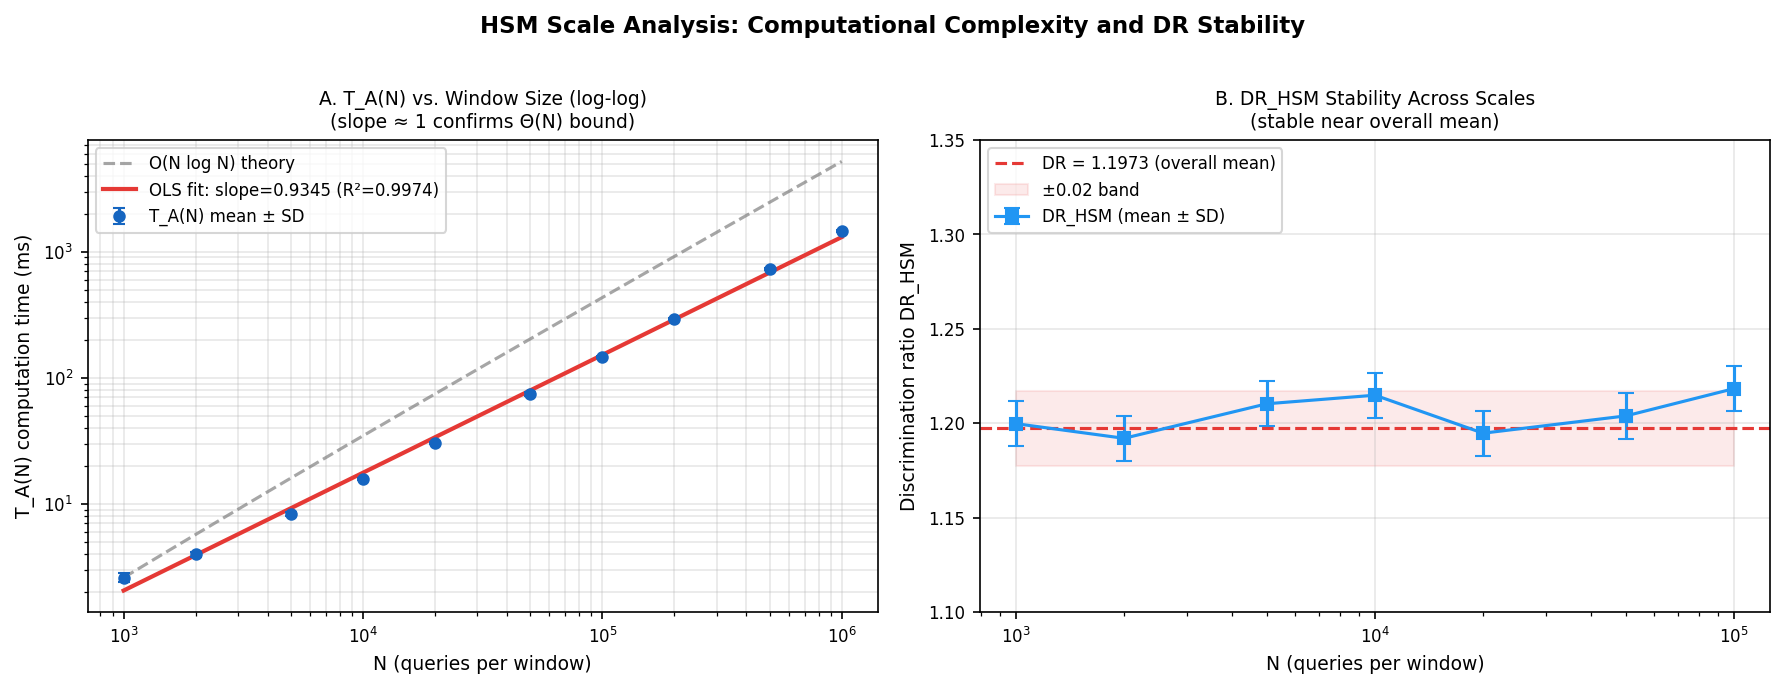
\includegraphics[width=\columnwidth]{figures/image8.png}
\caption{HSM scale analysis. (A) $T_A(N)$ vs.\ cardinality (log-log);
OLS $\beta\!=\!1.177$, $R^2\!=\!0.998$; dashed: $\Theta(N\log N)$ theory.
(B) $\mathrm{DR}_{\mathrm{HSM}}$ vs.\ $N$; per-SF Youden $J$ in
Table~\ref{tab:scale}.}
\label{fig:scale}
\end{figure}

%%─────────────────────────────────────────────────────────────
\section{Gate Sensitivity: Extended Results}\label{supp:gate}
%%─────────────────────────────────────────────────────────────

Table~\ref{tab:gate-sensitivity-supp} provides the full gate sensitivity
metrics across three scale factors, and Figure~\ref{fig:gate-sensitivity-supp}
visualises the margin $z$ and discriminability $d'$.

\begin{table}[htbp]\centering\scriptsize
\caption{Gate sensitivity ($\theta\!=\!0.75$, 10-block RCB).}
\label{tab:gate-sensitivity-supp}
\setlength{\tabcolsep}{3pt}
\begin{tabular}{@{}lccccccc@{}}
\toprule
\textbf{SF} & $\bar{h}_{\mathrm{st}}$ & $\sigma$ & GM & $z$ & FAP & $d'$ & Det.\\
\midrule
0.2  & 0.887 & 0.033 & 0.137 & 4.15 & 0/210 & 13.34 & 100\%\\
1.0  & 0.884 & 0.040 & 0.134 & 3.40 & 2/210 & 12.27 & 100\%\\
3.0  & 0.884 & 0.038 & 0.134 & 3.55 & 2/210 & 12.70 & 100\%\\
\bottomrule
\end{tabular}
\end{table}

\begin{figure}[htbp]\centering
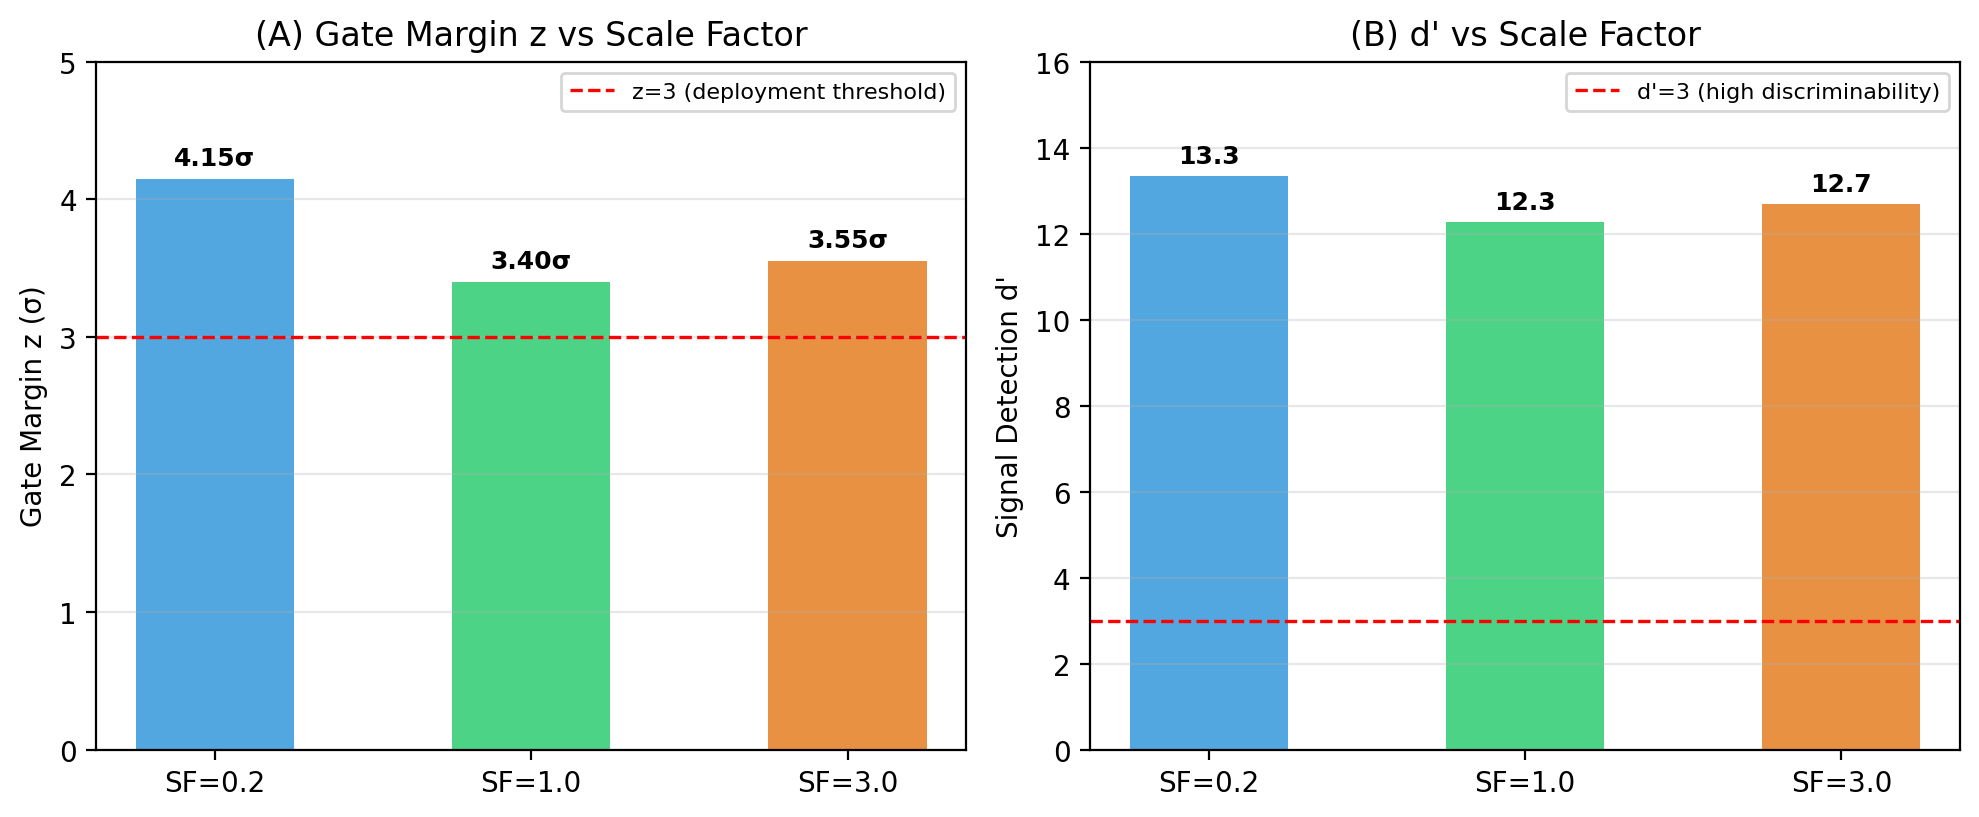
\includegraphics[width=\columnwidth]{figures/gate_sensitivity.png}
\caption{Gate sensitivity across scale factors ($z\!>\!3\sigma$ at all SFs; $d'\!>\!12$).}
\label{fig:gate-sensitivity-supp}
\end{figure}

%%─────────────────────────────────────────────────────────────
\section{$\theta$ Calibration: Cross-Engine ROC Analysis}\label{supp:theta-cal}
%%─────────────────────────────────────────────────────────────

Figure~\ref{fig:theta-cal-supp} presents the engine-specific threshold
calibration analysis discussed in the main paper's A-CE section.

\begin{figure}[htbp]\centering
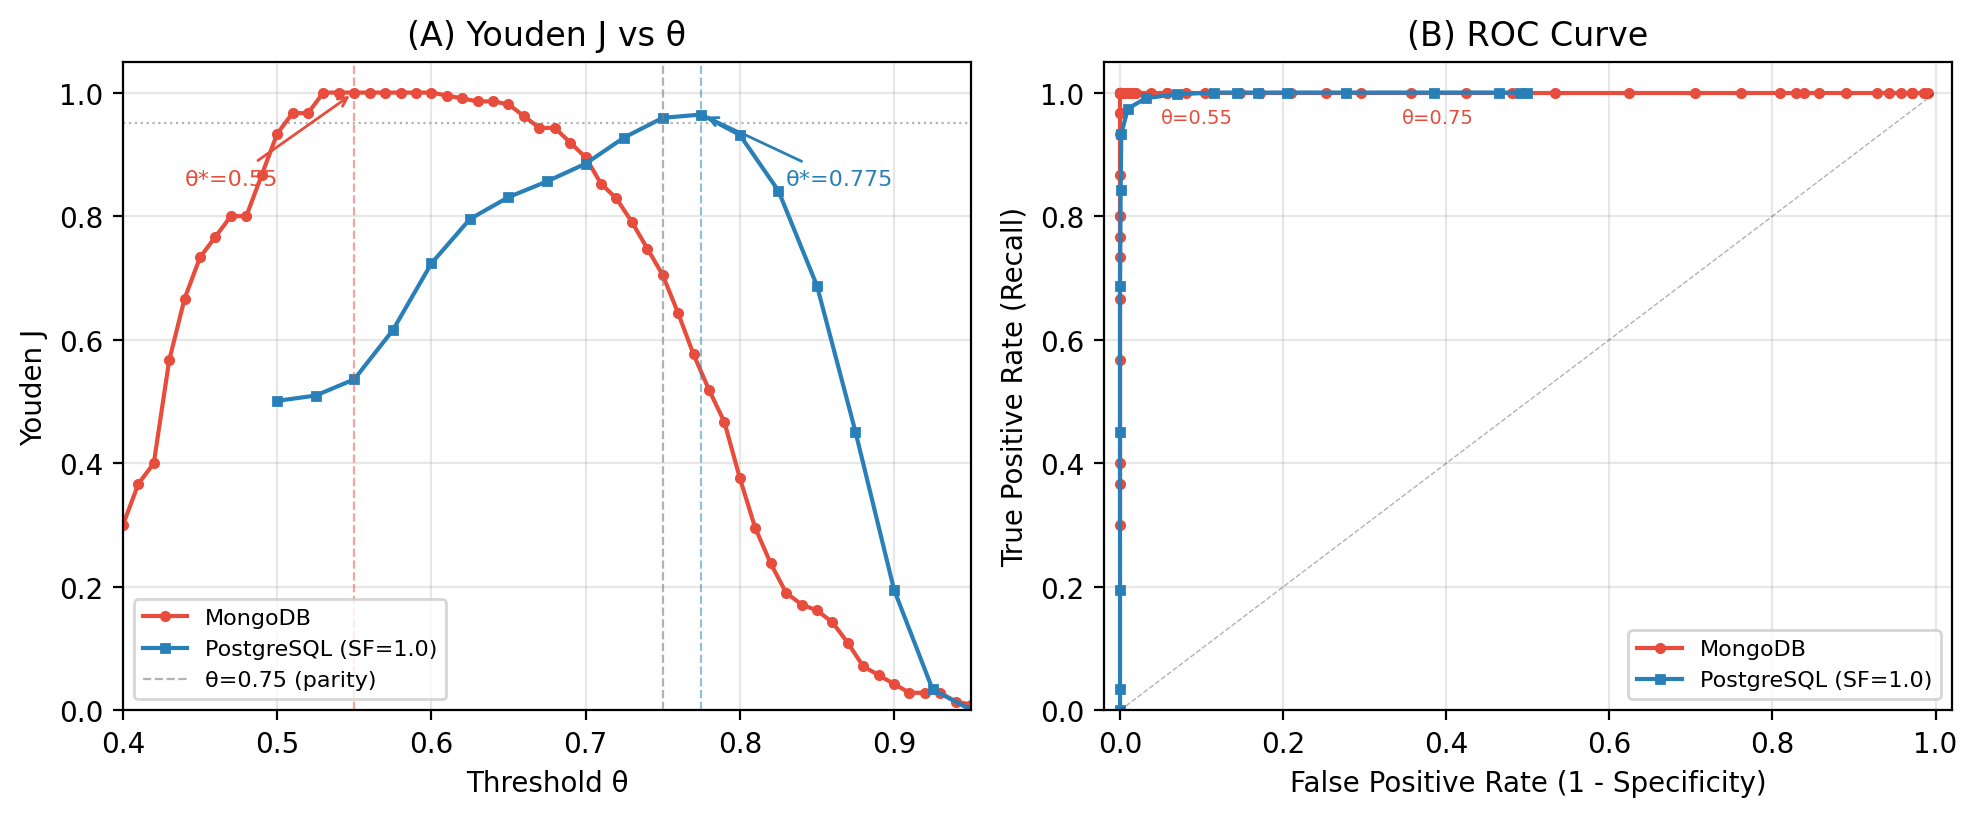
\includegraphics[width=\columnwidth]{figures/theta_calibration.png}
\caption{Engine-specific $\theta$ calibration. (A)~Youden $J$ vs.\ $\theta$:
MongoDB peaks at $\theta^*\!=\!0.55$, PostgreSQL at $\theta^*\!=\!0.775$.
(B)~ROC curves confirm high AUC for both engines; the operating-point
shift reflects data-model differences, not kernel failure.}
\label{fig:theta-cal-supp}
\end{figure}

\FloatBarrier
%%─────────────────────────────────────────────────────────────
\section*{Notation Summary}
%%─────────────────────────────────────────────────────────────

\begin{table}[h]\centering\small
\caption{Notation used in Supplementary Sections~I--XIII (Lemmas~1--4, Theorems~1--5, extended experiments, and additional analyses).}
\resizebox{\columnwidth}{!}{%
\begin{tabular}{@{}ll@{}}
\toprule
\textbf{Symbol} & \textbf{Definition}\\
\midrule
$W_A,W_B$       & Comparison workload windows\\
$\Npts=|W_A|+|W_B|$ & Total query events across both windows\\
$N$             & Database cardinality (rows in indexed table)\\
$\SR,\SV,\ST,\SA,\SPER$ & Five HSM dimension scores, each $\in[0,1]$\\
$w_R\!=\!0.25;\ w_V\!=\!w_T\!=\!w_A\!=\!0.20;\ w_P\!=\!0.15$ & Default dimension weights\\
$\dHSM=1-\SHSM$ & HSM distance function\\
$\thetastar$    & Optimal RETAIN/REBUILD decision threshold (Theorem~3)\\
$p_{\mathrm{stable}}$ & Probability HSM decides RETAIN on a window\\
$\hat{p}_{m}$   & Empirical RETAIN rate from $m$ window observations\\
$\eta_{m,\delta}$ & Hoeffding half-width $\sqrt{\log(2/\delta)/(2m)}$\\
$\Cdb=\sqrt{2}/2$ & db4 $\ell^{2}$-norm filter constant (Lemma~4)\\
$\varepsilon(M,\Npts,L)$ & DWT pattern-preservation error (Theorem~1)\\
$Q_{\min}(N)$   & Break-even query volume (Theorem~3)\\
\bottomrule
\end{tabular}}
\end{table}

\FloatBarrier
\bibliographystyle{plain}
\bibliography{references}

\end{document}
